\documentclass{article}
\usepackage[paperwidth=14cm,paperheight=5.4cm,margin=0.15cm]{geometry}
\usepackage{tikz}
\pagestyle{empty}
\pdfinfo{/Author (RISC-V CPU) /Creator () /Producer ()}
\begin{document}\noindent
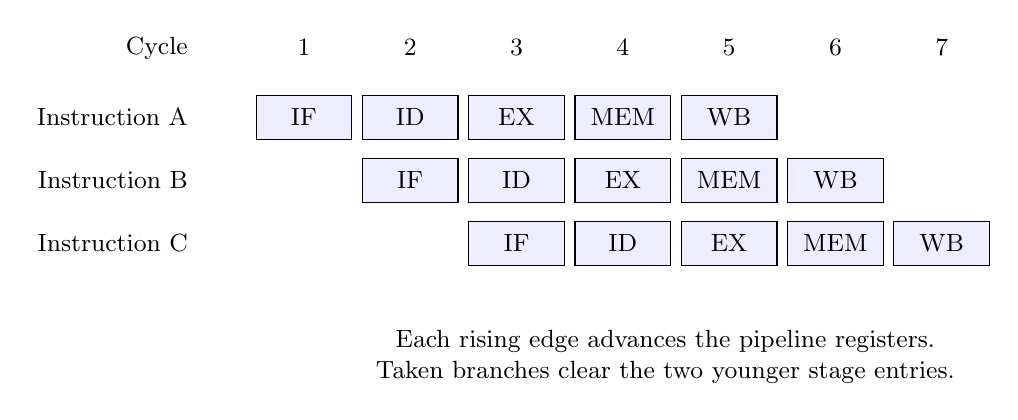
\begin{tikzpicture}[x=1.35cm,y=0.8cm,every node/.style={font=\small}]
\node[anchor=east] at (1,5.8) {Cycle};
\foreach \c in {1,...,7} \node at (\c+1,5.8) {\c};
\foreach \r/\name in {0/A,1/B,2/C} {
 \node[anchor=east] at (1,4.7-\r) {Instruction \name};
 \foreach \s/\name in {0/IF,1/ID,2/EX,3/MEM,4/WB} {
  \draw[fill=blue!7] (1.55+\r+\s,4.35-\r) rectangle (2.45+\r+\s,5.05-\r);
  \node at (2+\r+\s,4.7-\r) {\name};
 }
}
\node[align=center] at (5.4,0.9) {Each rising edge advances the pipeline registers.\\Taken branches clear the two younger stage entries.};
\end{tikzpicture}\end{document}
